\documentclass[11pt]{article}
\usepackage[utf8]{inputenc}
\usepackage[french]{babel}
\usepackage{graphicx}
\usepackage[T1]{fontenc}
%\usepackage{amss}
\usepackage{amsmath}
\usepackage{amsfonts}
\usepackage{amssymb}

\newcommand\comment{}
\def\N{\mathbb N}
\def\R{\mathbb R}
\def\Q{\mathbb Q}
\def\Z{\mathbb Z}
\begin{document}
\title{PARTIEL I31, 2015}
\date{}\maketitle
{\it Tous vos documents sont autorisés, mais pas la copie de votre voisin.
N'écrivez aucun programme.
Ecrivez lisiblement.
Répondez aux questions dans l'ordre, en indiquant le numéro de chaque question.
}




\section{Euclide et Bezout}

\smallskip

\begin{enumerate}
\item  En utilisant l'algorithme d'Euclide étendu, calculez le pgcd de 330 et 210 ainsi que les coefficients de Bezout  $u, v$~:
$$u\in \Z, v\in \Z \mbox{ tels que } 330\times u+210\times v=\mbox{PGCD}(330, 210)$$

Complétez le tableau ci-dessous. On rappelle que les coefficients $(u, v)$ de Bezout sont ceux pour lesquels $u^2 + v^2$ est le plus petit.


\item Donnez une formule avec un paramètre $t\in \Z$ permettant de générer toutes les paires d'entiers  $(u, v)$ telles
que $330u+210v=\mbox{PGCD}(330, 210)$.

\end{enumerate}

\medskip
%\begin{tabular}{|p{2cm}|p{2cm}|p{2cm}|p{2cm}|p{2cm}|p{2cm}|p{2cm}|}
$$
\begin{array}{|c|c|c|c|c|c|c|}
\hline 
\quad a\quad  &\quad  b\quad  & r=b\mbox{ mod }a & q=a\div b & \mbox{pgcd} & \quad u \quad & \quad v \quad \\ 
\hline 
330 & 210  & &   &   &   & \\
% & &    &   &   &   & \\
\hline
 & &    &   &   &   & \\
% 	 & &    &   &   &   & \\
\hline
 & &    &   &   &   & \\
%	 & &    &   &   &   & \\
\hline
  & &    &   &   &   & \\
%	  & &    &   &   &   & \\
\hline  
 & &    &   &   &   & \\
%	 & &    &   &   &   & \\
\hline
\end{array}
$$
%\end{tabular}




\section{Quizz}

\begin{enumerate}
\item Citez deux problèmes indécidables en informatique.

\item  Quand dit-on qu'un problème est difficile en informatique.

\item  Citez deux problèmes solubles en informatique, mais difficiles.

\item  Donnez deux algorithmes efficaces pour trier des nombres  en utilisant des comparaisons. Indiquez la complexité (en nombre de comparaisons) de ces deux algorithmes.

\item   Donnez le nom de trois algorithmes calculant les plus courts chemins dans un graphe.
\end{enumerate}

\section{Ordonnancement}

\begin{center}
\includegraphics[width=0.85\linewidth]{critique2.eps}
\end{center}

%\textbf{ajouter 0-0 et 5-7 dans les deux tâches du début ?}

Etant donnée la description des tâches donnée ci-dessus~: 

\begin{enumerate}

\item 
En calculant de Source vers Puits, complétez les dates au plus tôt (comme par exemple 0- et 5-).


Puis en calculant de  Puits vers Source, complétez les dates au plus tard (comme par exemple -0 et -7).

Soulignez le chemin critique.


\item Que faire si le graphe a plusieurs sommets sources (ou puits) ?

\item  Vous pouvez supposer que le graphe est acyclique, qu'il a un seul sommet source, un seul sommet puits, et que les durées sur les arcs sont non négatives.
Donnez la définition, en français, de la date au plus tôt. 
Prévoyez bien tous les cas~: sommet avec ou sans arc entrant ou sortant. 

\item   Donnez la définition, en français, de la date au plus tard.
Prévoyez bien tous les cas.

\item   Quand un sommet est-il critique~?

\end{enumerate}

\section{Dessinez le graphe d'un jeu de Nim}
Deux joueurs jouent à tour de rôle (Albert commence, Bertrand joue en second). Sur la table, il y a trois tas de pions~:
deux tas de 2 pions, et un tas de 1.

\smallskip
Chacun des joueurs choisit un tas (non vide) et  un seul,
et en retire un nombre entier strictement positif de pions~; il peut retirer  tous les pions du tas s'il le souhaite. 

\smallskip
Le premier joueur qui ne peut plus retirer de pions
a perdu.

\medskip
Vous utiliserez une représentation des états par niveaux: le niveau $n$ contient les états où la somme des nombres de pions vaut $n$ ($0 \le n \le 6 $). Un seul des états équivalents est représenté ($(2, 1, 1)=(1, 2, 1)=(1, 1, 2)$) et les $0$ inutiles sont éliminés.

Par exemple le niveau 2 contient
les deux  états~: $(2)$,  et $(1, 1)$. 

Un sommet est gagnant ssi le joueur qui y arrive peut toujours gagner, quels que soient les coups joués par l'adversaire.
Un sommet est perdant si et seulement si il n'est pas gagnant.

\begin{center}
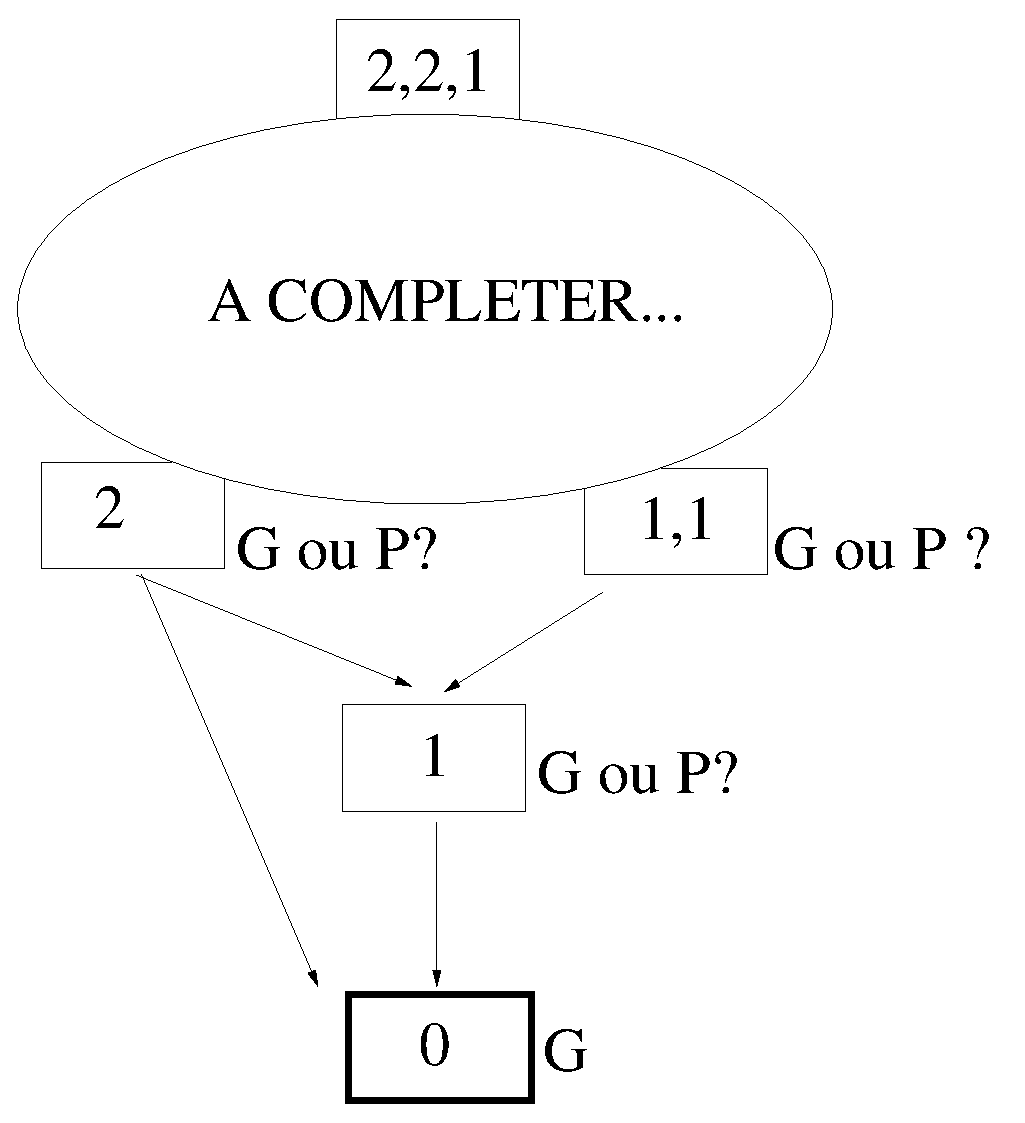
\includegraphics[width=0.65\linewidth]{nim2.eps}
\end{center}

\begin{enumerate}
\item Le schéma fourni ne contient que les niveaux 0, 1, 2. Ajoutez les 4 états manquants.


\item Sur le graphe, dessinez les arcs de tous les coups possibles~; il y a 16 arcs en tout~; chaque état  est représenté par un sommet~; un arc va d'un sommet $s$ à un sommet $t$ quand il est possible de passer en un coup de $s$ à $t$. 

\item Marquez chaque sommet G s'il est gagnant et P s'il est perdant. Epaississez le contour des sommets gagnants.

\item  Quel joueur, Albert ou Bertrand, est sûr de gagner, s'il joue intelligemment, bien sûr~?

\item  Décrivez l'algorithme que vous avez utilisé pour marquer les sommets G ou P.

\item  Dans un graphe orienté acyclique (c'est le cas ici), un noyau $N$ est 
un sous-ensemble de sommets du graphe tel que~: si  un sommet $s$ est dans $N$, tous ses successeurs (s'il en a) sont hors de $N$~; si $s$ est hors de $N$, alors il existe au moins un arc de $s$ vers un sommet $n$ qui se trouve dans $N$. 

Quel est le lien avec le problème précédent~? 

\end{enumerate}


\end{document}
